%----------------------------------------------------------------------------------------
%
% LaTeX-template for degree projects at LNU, Department of Computer Science
% Last updated by Johan Hagelbäck, Oct 2015
% Linnaeus University
%
% License: Creative Commons BY
%
%----------------------------------------------------------------------------------------

%----------------------------------------------------------------------------------------
%	Settings and configuration
%----------------------------------------------------------------------------------------

\documentclass[a4paper,12pt]{article}

\usepackage[T1]{fontenc}
\usepackage{times}
\usepackage[english]{babel}
\usepackage[utf8]{inputenc}
\usepackage{wallpaper}
\usepackage[absolute]{textpos}
\usepackage[top=2cm, bottom=2.5cm, left=3cm, right=3cm]{geometry}
\usepackage{appendix}
\usepackage[nottoc]{tocbibind}
\usepackage{enumerate}
\usepackage{array}
\newcolumntype{L}[1]{>{\raggedright\let\newline\\\arraybackslash\hspace{0pt}}m{#1}}

\setcounter{secnumdepth}{3}
\setcounter{tocdepth}{3}

\usepackage{sectsty}
\sectionfont{\fontsize{14}{15}\selectfont}
\subsectionfont{\fontsize{12}{15}\selectfont}
\subsubsectionfont{\fontsize{12}{15}\selectfont}
\usepackage[font=large, labelfont=bf]{caption}

\usepackage{csquotes} % Used to handle citations

\renewcommand{\thetable}{\arabic{section}.\arabic{table}}  
\renewcommand{\thefigure}{\arabic{section}.\arabic{figure}} 

%----------------------------------------------------------------------------------------
%	
%----------------------------------------------------------------------------------------
\newsavebox{\mybox}
\newlength{\mydepth}
\newlength{\myheight}

\newenvironment{sidebar}%
{\begin{lrbox}{\mybox}\begin{minipage}{\textwidth}}%
{\end{minipage}\end{lrbox}%
 \settodepth{\mydepth}{\usebox{\mybox}}%
 \settoheight{\myheight}{\usebox{\mybox}}%
 \addtolength{\myheight}{\mydepth}%
 \noindent\makebox[0pt]{\hspace{-20pt}\rule[-\mydepth]{1pt}{\myheight}}%
 \usebox{\mybox}}

%----------------------------------------------------------------------------------------
%	Title section
%----------------------------------------------------------------------------------------
\newcommand\BackgroundPic{
    \put(-2,-3){
    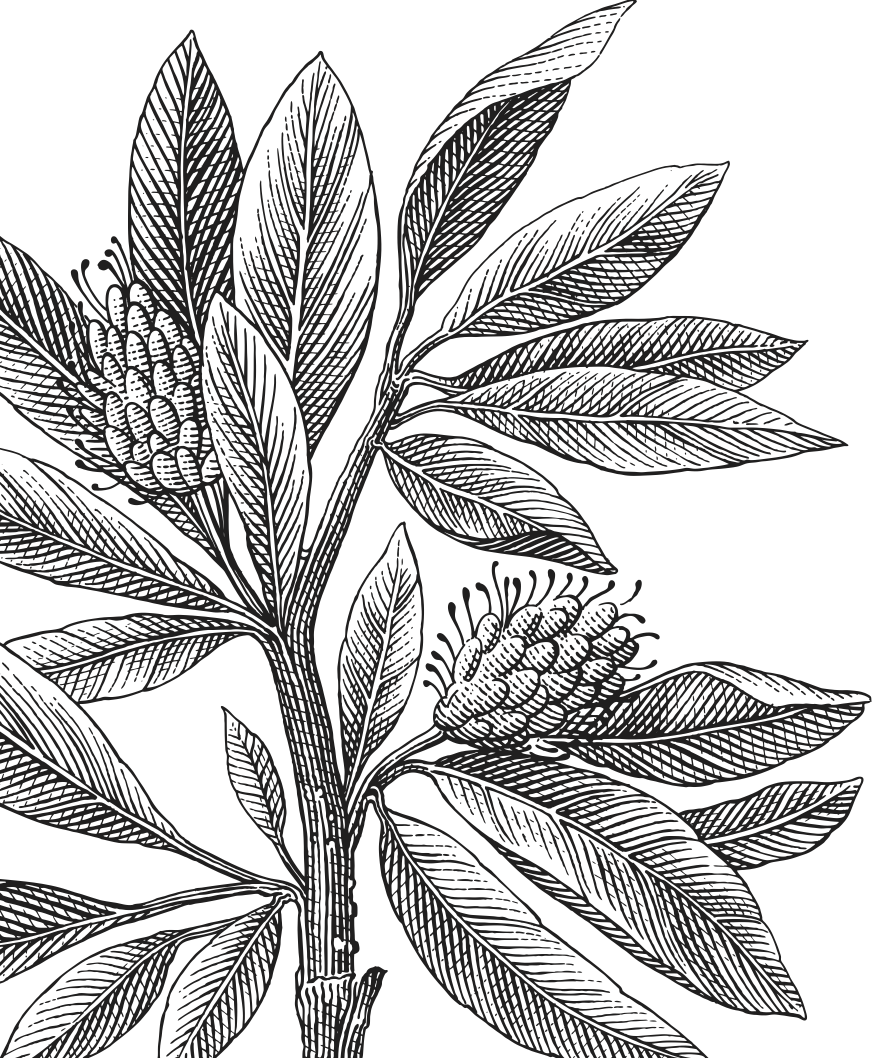
\includegraphics[keepaspectratio,scale=0.3]{img/lnu_etch.png} % Background picture
    }
}
\newcommand\BackgroundPicLogo{
    \put(30,740){
    
\includegraphics[keepaspectratio,scale=0.10]{img/logo.png} % Logo in upper left corner
    }
}

\title{	
\vspace{-8cm}
\begin{sidebar}
    \vspace{10cm}
    \normalfont \normalsize
    \Huge Report \\
    \vspace{-1.3cm}
\end{sidebar}
\vspace{3cm}
\begin{flushleft}
    \huge Project Course In Computer Science\\ 
    \it \LARGE - Deliveries Document
\end{flushleft}
\null
\vfill
\begin{textblock}{6}(10,13)
\begin{flushright}
\begin{minipage}{\textwidth}
\begin{flushleft} \large
\emph{Author:} Quasim Aljubarah, Michael Johansson, Tadas Lisauskas, Zeyuan Li, Robin Reijo and Robin Stempa\\ % Author
\emph{Supervisor:} Ola Petersson\\ % Supervisor
%\emph{Examiner:} Dr.~Mark \textsc{Brown}\\ % Examiner (course manager)
\emph{Semester:} VT 2016\\ % 
\emph{Subject:} 1DV508\\ % Subject area
\end{flushleft}
\end{minipage}
\end{flushright}
\end{textblock}
}

\date{} 

\begin{document}
\pagenumbering{gobble}
\newgeometry{left=5cm}
\AddToShipoutPicture*{\BackgroundPic}
\AddToShipoutPicture*{\BackgroundPicLogo}
\maketitle
\restoregeometry
\clearpage

\selectlanguage{english}

\tableofcontents

\newpage
\pagenumbering{gobble}
\pagenumbering{arabic}

%----------------------------------------------------------------------------------------
%
%	Here follows the actual text contents of the report.
%
%----------------------------------------------------------------------------------------
\section{Introduction}
In this document we will set the start and finishing date on our different requirements from the analysis document. We will choose which requirement that should be completed when and also in what order. 

\section{General requirements}
\begin{table}[htbp]
	\centering
	\caption{General requirements table}
	\label{my-label}
	\begin{tabular}{|l|L{8cm}|L{2.5cm}|L{2.5cm}|}
		\hline
		\textbf{ID} & \textbf{Requirements}                                                                                                                & Deadline & Status \\ \hline
		1           & The webshop must contain any number of products.                                                                                     &    Seminar 1      &        \\ \hline
		1.1         & All information about the products shall be stored in the database.                                                                  &     Seminar 1     &        \\ \hline
		1.1.1       & \begin{tabular}[c]{@{}l@{}}product must have: \\ -Product name\\ -Category\\ -Quantity\\ -Price\\ -Description\\ -Image\end{tabular} &    Seminar 1      &        \\ \hline
		1.1.2       & All products will be pre-defined to categories (Monitors,Computers, Etc.)                                                            &     Seminar 2     &        \\ \hline
		1.2         & When an order is placed it must be added to the database                                                                             &   Seminar 3       &        \\ \hline
		1.2.1       & When an order is placed the quantity of the products must change                                                                     &    Seminar 3      &        \\ \hline
	\end{tabular}
\end{table}

\newpage

\section{Customer requirements}
\begin{table}[htbp]
	\centering
	\caption{Customer requirements table}
	\label{my-label}
	\begin{tabular}{|l|L{8cm}|L{2.5cm}|L{2.5cm}|}
		\hline
		\textbf{ID}    & \textbf{Requirement}                                                                                                                                                                          & Deadline & Status \\ \hline
		\textbf{2}     & The customer must be able to browse the products in the following ways:\newline -Browse all products\newline -Search for a product\newline -Show products in a category &  seminar 4       &        \\ \hline
		\textbf{2.1}   & It must be possible to click on a product to see more details about it.                                                                                                                       &    Seminar 4      &        \\ \hline
		\textbf{2.2}   & The customer must be able to put a product in a cart.                                                                                                                                         &   Seminar 3       &        \\ \hline
		\textbf{2.2.1} & The customer must be able to view the products in the cart.                                                                                                                                   &     Seminar 3    &        \\ \hline
		\textbf{2.2.2} & The customer must be able to change the quantity of a product in the cart.                                                                                                              &   Seminar 3       &        \\ \hline
		\textbf{2.2.3} & The customer must be able to remove a product from the cart with one click with any quantity.                                                     &     Seminar 3     &        \\ \hline
		\textbf{2.3}   & The customer must be able to place an order   .                                                                                                                                               &     Seminar 5     &        \\ \hline
		\textbf{2.3.1} & When placing an order, a form must be shown where the customer enters his/her contact details (email, address, phone number).                      &    Seminar 5      &        \\ \hline
		\textbf{2.3.2} & When an order is finalized the customer must receive an auto-generated order number.                                                                                                          &  Seminar 5        &        \\ \hline
		\textbf{2.3.3} & The customer must be able to check the status of his/her order from the order number.                                                                                                         &   Seminar 5       &        \\ \hline
	\end{tabular}
\end{table}

\newpage

\section{Administrator requirements}
\begin{table}[htbp]
	\centering
	\caption{Administrator requirements table}
	\label{my-label}
	\begin{tabular}{|l|L{8cm}|L{2.5cm}|L{2.5cm}|}
		\hline
		\textbf{ID} & \textbf{Requirement}                                                       & Deadline & Status \\ \hline
		3           & The webshop shall have an Admin system where an administrator can log on   &   Seminar 1       &        \\ \hline
		3.1         & Administrator accounts and passwords shall be stored in the database.      &  Seminar 1        &        \\ \hline
		3.2         & An administrator must be able to add a new product                         &  Seminar 1        &        \\ \hline
		3.2.1       & An administrator must be able to remove a product                          &     Seminar 1     &        \\ \hline
		3.2.2       & An administrator must be able to change information about a product        &   Seminar 1       &        \\ \hline
		3.2.3       & An administrator must be able to add a category                            &     Seminar 2     &        \\ \hline
		3.2.4       & An administrator must be able to remove a category                         &     Seminar 2     &        \\ \hline
		3.2.5       & An administrator must be able to change information about a category       &   Seminar 2       &        \\ \hline
		3.3         & An administrator must be able to add a new administrator account           &     Seminar 4     &        \\ \hline
		3.3.1       & An administrator must be able to remove a administrator account            &    Seminar 4      &        \\ \hline
		3.4         & An administrator must be able to view all orders                           &     Seminar 3     &        \\ \hline
		3.4.1       & An administrator must be able update the order status on every order       &   Seminar 5       &        \\ \hline
		3.4.2       & The order status can only be New, Shipped, Delayed, Delivered and Returned &     Seminar 5     &        \\ \hline
		\end{tabular}
		\end{table}
		
\section{Conclusion}
We choose to start with the administrator pages and implementing the products. We also choose to have the sixth seminar to finishing touches and so we have a seminar to fall back on if there is any problems along the way.

\end{document}
